\chapter{Allen--Cahn crystallization}
\label{ch:p6}

\begin{keybox}
\textbf{Key idea.} Crystallinity is a \emph{non-conserved} order parameter
--- crystal can be created, unlike composition --- so it obeys
\emph{Allen--Cahn} (non-conserved gradient flow), not Cahn--Hilliard. A
crystal grows below the melting point and melts above it; the growth-front
\emph{velocity} rises with undercooling; a \emph{critical radius}
separates growing from redissolving seeds; and the way the crystalline
fraction advances in time is the Avrami (JMAK) law.
\end{keybox}

\begin{keybox}
\textbf{Learning objectives.} By the end you can: write the non-conserved
Allen--Cahn flow for $\psi$ and explain why crystal need not be conserved;
predict the sign of $\text{drive}=\Delta h(T/T_m-1)$ and hence grow vs
melt; measure $v(\Delta T)$ and explain its monotone rise (constant
mobility, no transport maximum); derive and bracket the critical radius
$r^\ast\propto\sigma/|\text{drive}|$; and fit the Avrami exponent
$n\pm$CI, explaining why finite pre-placed seeds give $n$ below the ideal
value.\\[2pt]
\textbf{Prerequisites.} Non-conserved gradient flows, the Gibbs--Thomson
balance, least-squares fitting with an uncertainty; Chapter~\ref{ch:p1}
(free-energy/gradient-flow language and the measure-with-uncertainty
habit).\\[2pt]
\textbf{Expected cost.} Any CUDA GPU, 2-D, $<1$\,GB device memory;
solver \code{cuDSS} (documented \code{splu} fallback). Quick mode
comparable to P1's measured $\approx75$\,s wall (RTX~6000 Ada, mostly
kernel compile); reference (four-experiment battery) a few minutes;
research (\code{--level 6}) tens of minutes.
\end{keybox}

\section{The model}

Let $\psi\in[0,1]$ be the local crystallinity of a crystallizable species.
Its non-conserved gradient flow is
%
\begin{equation}
  \dd{\psi}{t} = -L_\psi\Big[\dd{f}{\psi} - \varepsilon^2\grad^2\psi\Big],
\end{equation}
%
with the crystallization free energy (the 2310.11844 ``r14'' form,
PCBM-class energetics)
%
\begin{equation}
  f_{\text{cr}} = \phi\big[q(\psi)\,\Delta\sigma + p(\psi)\,\text{drive}\big],
  \quad q=\psi^2(1-\psi)^2,\quad p=\psi^2(3-2\psi),
\end{equation}
%
and the Turnbull undercooling driving force
%
\begin{equation}
  \text{drive} = \Delta h\,(T/T_m - 1).
\end{equation}
%
$q(\psi)$ is a double-well barrier separating amorphous ($\psi=0$) from
crystalline ($\psi=1$); $p(\psi)$ interpolates the driving; $L_\psi$ sets
the growth rate; $\varepsilon^2$ the crystal-interface width.

\begin{keybox}
\textbf{The melting point sets the sign.} $\text{drive}\propto(T/T_m-1)$
is \emph{negative} for $T<T_m$ (so $\psi\to1$ lowers $f$: the crystal
\emph{grows}) and \emph{positive} for $T>T_m$ (the crystal \emph{melts}).
$T_m=\ensuremath{\PsixTm}$~K here (materials.yaml, PCBM class). $\Delta h$
is the crystallization enthalpy, $\Delta\sigma$ the barrier height,
$L_\psi$ the kinetic prefactor, $\varepsilon^2$ the gradient penalty
(crystal interface width $\sim\sqrt{\varepsilon^2}$).
\end{keybox}

\begin{keybox}
\textbf{Measuring crystallinity: quadrature, not a threshold.} The primary
crystalline content is the \emph{quadrature} average
$\langle\psi\rangle = \int\psi\,\dV / \int\dV$, evaluated at the assembly
Gauss points (\code{diffsim.diagnostics.conservation}). It counts partial
(diffuse-interface) crystallinity honestly. A thresholded area fraction
($\psi>0.5$) is reported \emph{secondarily}, together with its sensitivity
to the cut ($0.4$/$0.5$/$0.6$), because a hard cut discards the interface
and depends on where you place it.
\end{keybox}

\section{Interface velocity and the critical radius}

Below $T_m$ a crystal front advances at a roughly constant velocity
$v$; we measure it as $v=\mathrm{d}r_{\rm eff}/\mathrm{d}t$ with
$r_{\rm eff}=\sqrt{\langle\psi\rangle_{\rm area}/\pi}$ over the pre-fill
window. Because the mobility $L_\psi$ here is \emph{constant} (no
thermally-activated hopping), $v$ rises \emph{monotonically} with the
undercooling $\Delta T=T_m-T$ (measured
$v=\ensuremath{\PsixVmild}\to\ensuremath{\PsixVdeep}$ as
$\Delta T=\ensuremath{\PsixdTmild}\to\ensuremath{\PsixdTdeep}$). Real
crystallization has a \emph{maximum} at intermediate $\Delta T$ because
molecular transport freezes out on deep cooling --- reproducing that
requires an activated $L_\psi(T)$, a labelled modelling extension
(Exercise~1), not the constant-mobility physics implemented here.

A curved seed pays interface energy $\sim 2\pi r\,\sigma$ while gaining
bulk energy $\sim \pi r^2\,|\text{drive}|$, so
$\mathrm{d}F/\mathrm{d}r=0$ at a \emph{critical radius}
%
\begin{equation}
  r^\ast \;\sim\; \frac{\sigma}{|\text{drive}|}
        \;\propto\; \frac{1}{|\,\Delta h\,(T/T_m-1)\,|}.
\end{equation}
%
Seeds larger than $r^\ast$ grow; smaller ones redissolve (the
Gibbs--Thomson floor). Deeper undercooling raises $|\text{drive}|$ and so
\emph{lowers} $r^\ast$. We bracket $r^\ast$ by seeding a range of radii
and classifying grow/shrink at two undercoolings: at $T=\ensuremath{\PsixTdeep}$~K
(deep) $r^\ast\approx\ensuremath{\PsixRstarDeep}$, at
$T=\ensuremath{\PsixTmild}$~K (mild) $r^\ast\approx\ensuremath{\PsixRstarMild}$.
The measured ratio $\ensuremath{\PsixRstarRatioMeas}$ agrees in sense (and
order of magnitude) with the Gibbs--Thomson prediction
$|\text{drive}_{\rm deep}|/|\text{drive}_{\rm mild}|=\ensuremath{\PsixRstarRatioPred}$;
the gap is honest --- finite-time classification, a weakly $T$-dependent
effective $\sigma$, and the $\phi$-coupling all enter.

\section{Growth kinetics: the Avrami law}

With athermal nuclei placed at $t=0$ growing at velocity $v$, the
crystalline area of each grain grows like $(vt)^2$ in 2-D before grains
impinge, so the crystalline \emph{fraction} follows the
Johnson--Mehl--Avrami--Kolmogorov (JMAK) law
%
\begin{equation}
  X(t) = 1 - \exp\!\big[-(kt)^n\big].
\end{equation}
%
Because our nuclei are \emph{finite pre-placed} seeds (point seeds are
sub-critical and redissolve --- exactly the $r^\ast$ floor above), the
film starts with a crystalline baseline $X_0$. We remove it with the
\emph{generalized-JMAK} conversion $X^\ast=(X-X_0)/(1-X_0)$ and fit
%
\begin{equation}
  \ln[-\ln(1-X^\ast)] = n\ln t + n\ln k
\end{equation}
%
by least squares over the pre-impingement window
$\ensuremath{0.05}<X^\ast<\ensuremath{0.9}$, reporting the window, the
number of points, $R^2$, and a $95\%$ CI on $n$. The ideal exponents are
$n\approx3$ for point nuclei appearing over time and $n\approx2$ for
pre-existing 2-D nuclei; finite pre-placed seeds give an effective $n$
\emph{below} $2$ because the seeds start with area and the early $t^2$
regime is foreshortened.

\begin{keybox}
\textbf{Accelerated parameters.} The Avrami run uses $T=250$~K and
$L_\psi=11$, which are \emph{pedagogical accelerated} values (not the
physical PCBM rate): they let $X$ sweep the full $(0,1)$ range inside a
short run so the double-log fit has a real window. Likewise
\textbf{orientation $\theta$ is a fixed grain \emph{label}, not an evolved
field} (\code{theta\_mode="frozen"}, $\alpha_\theta=\beta_\theta=0$): there
is \emph{no} grain-boundary energy and \emph{no} $\theta$ dynamics here.
\code{grain\_labels} merely reads the frozen $\theta$ plateaus to count
crystals. Evolving $\theta$ (Kobayashi--Warren--Carter grain boundaries) is
the coupled concept of Chapter~\ref{ch:p7}.
\end{keybox}

\section{Run it}

\begin{runbox}
\textbf{Run it.}
\begin{lstlisting}
cd physics/06_allen_cahn_crystallization
python run.py            # grow/melt + v(dT) + r* + Avrami, then checks
\end{lstlisting}
It runs the four-experiment battery, writes \file{outputs/results.json},
and checks it against \file{baseline.yaml} (tolerance-based). Compare with
\file{EXPECTED.md} and the figures.
\end{runbox}

\paragraph{What you should see.} Below the melting point ($T=333$~K) the
seeded disc \emph{grows} (quadrature crystallinity
$\ensuremath{\PsixGrowStart}\to\ensuremath{\PsixGrowEnd}$, a factor
$\ensuremath{\PsixGrowRatio}$, drive $\ensuremath{\PsixGrowDrive}$); above
it ($T=700$~K, drive $\ensuremath{\PsixMeltDrive}$) it \emph{melts}
($\to\ensuremath{\PsixMeltEnd}$). The growth-front velocity rises with
undercooling, the critical radius shrinks with it, and the multi-nucleus
run reaches $\langle\psi\rangle_{\rm end}=\ensuremath{\PsixAvramiXqend}$
($X_{\psi>0.5}=\ensuremath{\PsixAvramiXend}$) from $\ensuremath{\PsixSeeds}$
nuclei ($\ensuremath{\PsixGrains}$ grains resolved), with a
baseline-corrected Avrami exponent
$n=\ensuremath{\PsixAvramiN}\pm\ensuremath{\PsixAvramiCI}$
($R^2=\ensuremath{\PsixAvramiRsq}$, $X_0=\ensuremath{\PsixAvramiXzero}$).

% --- generated by gen_figures.py ---
\begin{figure}[h]\centering
  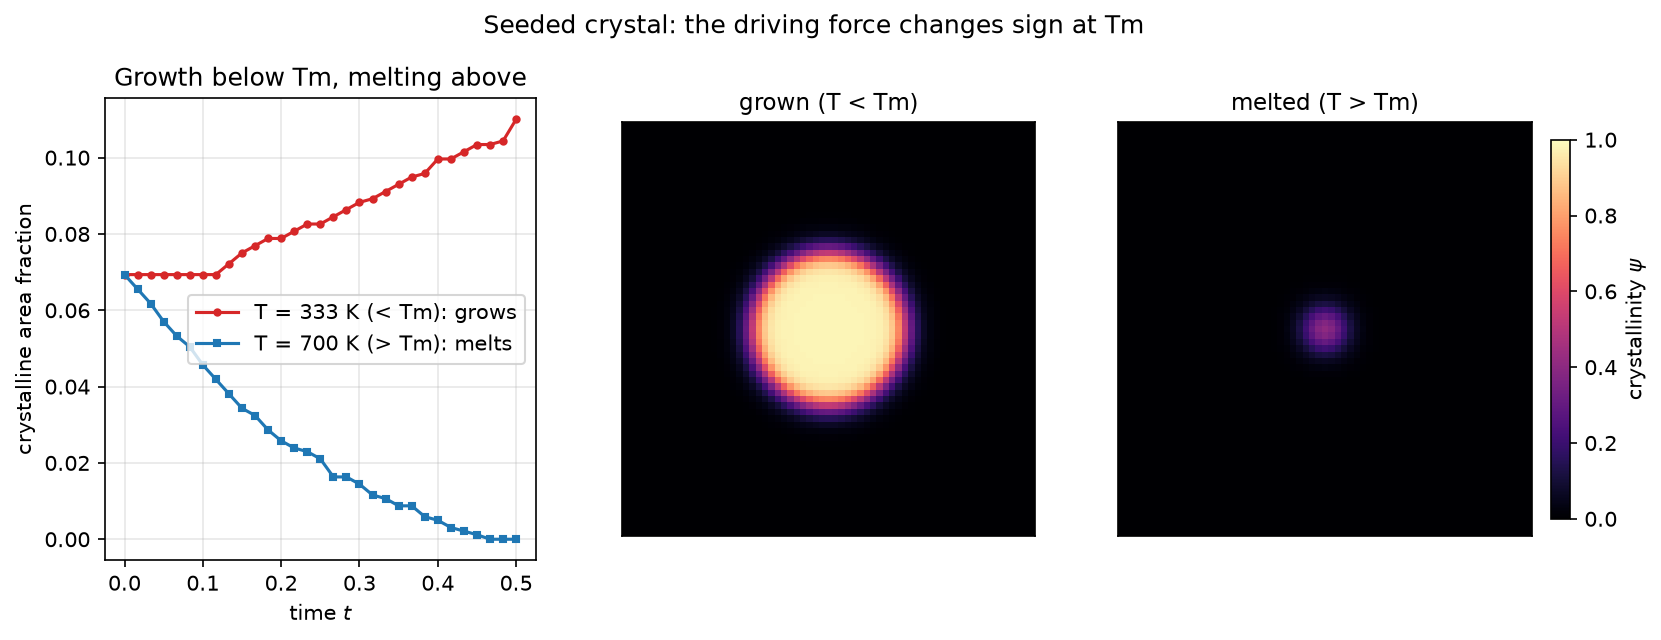
\includegraphics[width=\linewidth]{figures/p6_grow_melt.png}
  \caption{A seeded crystal grows below $T_m$ and melts above it (left:
    quadrature crystallinity $\langle\psi\rangle$ vs time; right: the final
    $\psi$ fields). The driving force changes sign at the melting point.}
  \label{fig:p6growmelt}
\end{figure}

\begin{figure}[h]\centering
  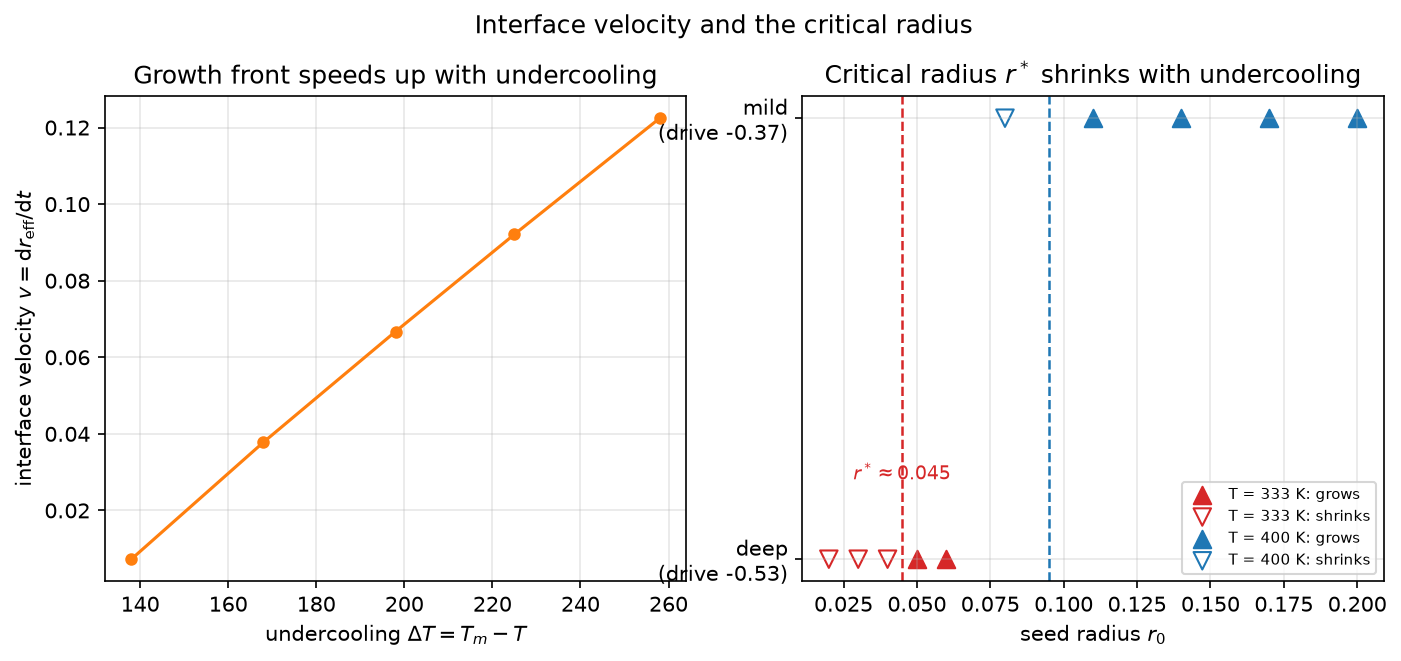
\includegraphics[width=\linewidth]{figures/p6_kinetics.png}
  \caption{Left: the growth-front interface velocity $v$ rises
    monotonically with undercooling $\Delta T=T_m-T$ (constant mobility ---
    no thermal-transport maximum). Right: the critical radius $r^\ast$
    brackets --- seeds above $r^\ast$ grow ($\triangle$), below it shrink
    ($\triangledown$) --- and $r^\ast$ shrinks as the undercooling deepens.}
  \label{fig:p6kinetics}
\end{figure}

\begin{figure}[h]\centering
  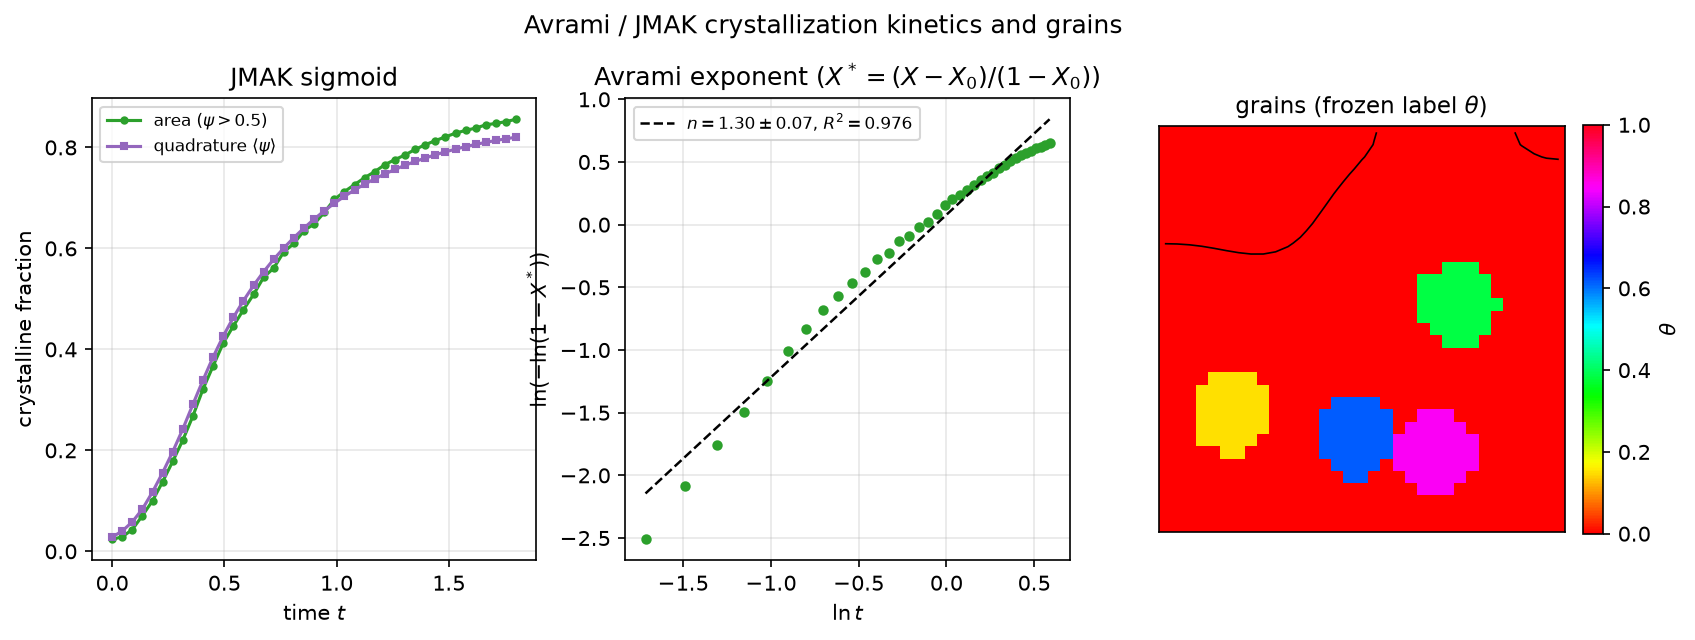
\includegraphics[width=\linewidth]{figures/p6_avrami.png}
  \caption{Avrami/JMAK kinetics: the sigmoidal crystalline fraction (left,
    quadrature and thresholded), the baseline-corrected double-log
    linearization whose slope is the Avrami exponent $n\pm$CI with its
    $R^2$ (middle), and the grains coloured by the frozen orientation
    label $\theta$ with the crystal outline (right).}
  \label{fig:p6avrami}
\end{figure}

\begin{keybox}
\textbf{Measured self-check} (level 5, cuDSS; tolerance-checked in
\file{baseline.yaml}).
\begin{center}\small
\begin{tabular}{lc}
\toprule
grow ($T<T_m$): $\langle\psi\rangle$ start $\to$ end & $\ensuremath{\PsixGrowStart} \to \ensuremath{\PsixGrowEnd}$ ($\ensuremath{\PsixGrowRatio}\times$) \\
melt ($T>T_m$): $\langle\psi\rangle$ end & $\ensuremath{\PsixMeltEnd}$ \\
critical radius $r^\ast$ (deep $\to$ mild) & $\ensuremath{\PsixRstarDeep} \to \ensuremath{\PsixRstarMild}$ \\
Avrami exponent $n$ & $\ensuremath{\PsixAvramiN}\pm\ensuremath{\PsixAvramiCI}$ ($R^2=\ensuremath{\PsixAvramiRsq}$) \\
crystalline fraction $\langle\psi\rangle_{\text{end}}$ & $\ensuremath{\PsixAvramiXqend}$ \\
nuclei $\to$ grains resolved & $\ensuremath{\PsixSeeds} \to \ensuremath{\PsixGrains}$ \\
\bottomrule
\end{tabular}
\end{center}
\end{keybox}

\section{Code walk-through}

\paragraph{1. The crystallizing stepper.} \code{MultiPhaseStepper(dm,
M=1, K=1, ..., bulk="r14")} adds one crystallinity field $\psi$ (and its
frozen orientation label $\theta$) to one composition. \code{dsig},
\code{dh}, \code{Tm}, \code{eps2}, \code{L\_psi} are the coefficients above.

\paragraph{2. Quadrature crystallinity.} \code{quad\_mean\_psi} evaluates
$\psi$ at the Gauss points and forms $\int\psi\,\dV/\int\dV$ with the
assembly quadrature weights --- the primary crystallinity measure.

\paragraph{3. Interface velocity and $r^\ast$.}
\code{run\_interface\_velocity} fits $v=\mathrm{d}r_{\rm eff}/\mathrm{d}t$;
\code{run\_critical\_radius} classifies a radius sweep into grow/shrink and
brackets $r^\ast$.

\paragraph{4. The Avrami fit.} \code{\_fit\_avrami} baseline-corrects
$X\to X^\ast$, linearizes over the window, and returns $n$, $k$, $R^2$ and
the CI; the grains come from \code{grain\_labels} (a $\theta$-plateau
watershed on the frozen label).

\section{Explore on your own}

\question{Replace the constant $L_\psi$ with an activated mobility
$L_\psi(T)=L_0\exp[-E_a/T]$. Does $v(\Delta T)$ now develop a maximum at
intermediate undercooling (transport-limited on deep cooling)? Where does
the peak sit relative to the constant-mobility curve of
Figure~\ref{fig:p6kinetics}?}

\question{Change the number of pre-placed nuclei and re-fit $n$ (with its
CI). Does $n$ stay near its finite-seed value, or move toward $2$/$3$ as
you shrink the seeds toward point nuclei? What does $n$ tell you about the
nucleation mode?}

\question{Sweep $\varepsilon^2$, measure the crystal interface width, and
confirm the $\sqrt{\varepsilon^2}$ scaling. Relate the width to the mesh
spacing --- when is the crystal interface under-resolved, and how does that
bias $r^\ast$?}

\question{Give two seeds \emph{different} orientation labels $\theta$ and
let them grow into contact. With the frozen $\theta$ here they simply
merge into one $\psi$ blob; adding grain-boundary energy (an evolving
$\theta$) is the coupled orientation dynamics of Chapter~\ref{ch:p7}.}

\question{The crystal expels the amorphous component as it grows (the
$\phi$ field). Measure the composition inside vs outside the crystal ---
this is the crystallization-driven demixing that Chapter~\ref{ch:p7}
makes central.}

% ====================================================================
